\documentclass[11pt]{beamer}
\usepackage[utf8]{inputenc}
\usepackage{graphicx, epsfig}
\usepackage{amsmath,mathrsfs,amsfonts,amssymb}
%\usepackage{subfig}
\usepackage{floatflt}
\usepackage{epic,ecltree}
\usepackage{mathtext}
\usepackage{fancybox}
\usepackage{fancyhdr}
\usepackage{multirow}
\usepackage{enumerate}
\usepackage{epstopdf}
\usepackage{multicol}
\usepackage{algorithm}
\usepackage[noend]{algorithmic}
\usepackage{tikz}
\usepackage{blindtext}
\usetheme{default}%{default}%{Singapore}%{Warsaw}%{Warsaw}%{Darmstadt}
\usecolortheme{default}
\setbeamerfont{title}{size=\Huge}
\setbeamertemplate{footline}[page number]{}


\makeatletter
\newcommand\HUGE{\@setfontsize\Huge{35}{40}}
\makeatother    

\setbeamerfont{title}{size=\HUGE}
\beamertemplatenavigationsymbolsempty

% latin bold lower
\newcommand{\ba}{\mathbf{a}} 
\newcommand{\bc}{\mathbf{c}} 
\newcommand{\be}{\mathbf{e}} 
\newcommand{\bh}{\mathbf{h}} 
\newcommand{\bp}{\mathbf{p}} 
\newcommand{\bt}{\mathbf{t}} 
\newcommand{\bs}{\mathbf{s}} 
\newcommand{\bu}{\mathbf{u}} 
\newcommand{\bv}{\mathbf{v}} 
\newcommand{\bw}{\mathbf{w}} 
\newcommand{\bx}{\mathbf{x}} 
\newcommand{\by}{\mathbf{y}} 
\newcommand{\bz}{\mathbf{z}} 

% latin bold upper
\newcommand{\bA}{\mathbf{A}} 
\newcommand{\bB}{\mathbf{B}} 
\newcommand{\bC}{\mathbf{C}} 
\newcommand{\bI}{\mathbf{I}} 
\newcommand{\bL}{\mathbf{L}} 
\newcommand{\bM}{\mathbf{M}} 
\newcommand{\bQ}{\mathbf{Q}} 
\newcommand{\bT}{\mathbf{T}} 
\newcommand{\bU}{\mathbf{U}} 
\newcommand{\bV}{\mathbf{V}} 
\newcommand{\bW}{\mathbf{W}} 
\newcommand{\bX}{\mathbf{X}} 
\newcommand{\bY}{\mathbf{Y}} 
\newcommand{\bZ}{\mathbf{Z}} 

% latin cal upper
\newcommand{\cG}{\mathcal{G}} 
\newcommand{\cL}{\mathcal{L}} 
\newcommand{\cN}{\mathcal{N}} 
\newcommand{\cS}{\mathcal{S}} 
\newcommand{\cT}{\mathcal{T}} 
\newcommand{\cW}{\mathcal{W}} 
\newcommand{\cX}{\mathcal{X}} 
\newcommand{\cZ}{\mathcal{Z}} 

% latin bb upper
\newcommand{\bbE}{\mathbb{E}} 
\newcommand{\bbI}{\mathbb{I}} 
\newcommand{\bbP}{\mathbb{P}} 
\newcommand{\bbR}{\mathbb{R}} 

% greek bold lower
\newcommand{\bepsilon}{\boldsymbol{\epsilon}} 
\newcommand{\btheta}{\boldsymbol{\theta}} 
\newcommand{\blambda}{\boldsymbol{\lambda}} 
\newcommand{\bpi}{\boldsymbol{\pi}} 
\newcommand{\bmu}{\boldsymbol{\mu}} 
\newcommand{\bsigma}{\boldsymbol{\sigma}} 
\newcommand{\bphi}{\boldsymbol{\phi}} 

% greek bold upper
\newcommand{\bSigma}{\boldsymbol{\Sigma}} 

\DeclareMathOperator*{\argmin}{arg\,min}
\DeclareMathOperator*{\argmax}{arg\,max}
\newcommand{\createdgmtitle}[1]{\title[\hbox to 56mm{Mathematical Forecasting Methods \hfill\insertframenumber\,/\,\inserttotalframenumber}]
	{\vspace{1.5\cm} \\ Mathematical Forecasting Methods \\ {\Huge Лекция #1}}
	\author{}
	\institute{
	МФТИ
	} 
	\date{Осень, 2023}
}

\newcommand\myfootnote[1]{%
  \tikz[remember picture,overlay]
  \draw (current page.south west) +(1in + \oddsidemargin,0.5em)
  node[anchor=south west,inner sep=0pt]{\parbox{\textwidth}{%
      \rlap{\rule{10em}{0.4pt}}\raggedright\scriptsize \textit{#1}}};}

\newcommand\myfootnotewithlink[2]{%
  \tikz[remember picture,overlay]
  \draw (current page.south west) +(1in + \oddsidemargin,0.5em)
  node[anchor=south west,inner sep=0pt]{\parbox{\textwidth}{%
      \rlap{\rule{10em}{0.4pt}}\raggedright\scriptsize\href{#1}{\textit{#2}}}};}
\createdgmtitle{2}
\usepackage{tikz}
\usepackage[english,russian]{babel}
\usepackage[labelformat=empty]{caption}
\usetikzlibrary{arrows,shapes,positioning,shadows,trees}
\newcommand*{\defeq}{\stackrel{\text{def}}{=}}

%--------------------------------------------------------------------------------
\begin{document}
%--------------------------------------------------------------------------------
\begin{frame}[noframenumbering,plain]
%\thispagestyle{empty}
\titlepage
\end{frame}
%=======
\begin{frame}{Временной ряд}
\begin{itemize}
\item \textbf{Временной ряд} --- это совокупность значения параметра $\{x_1, x_2,...,x_T\}= \{ x_t \}_{t=1}^T$, изменяющегося во времени,  через равные промежутки времени.

\item \textbf{Задача прогнозирования}: найти функции $f_{T,d}$:
\begin{equation*}
x_{T+d} \approx f_{T,d}(x_1,...x_T;w) =: \hat{x}_{T+d}, 
\end {equation*}
где $f_{T,d}$ --- модель временного ряда, $d =1,...,D$ --- горизонт прогнозирования.
\item \textbf{Минимизация квадратов ошибок} (МНК):
    \begin{equation*}
        Q_t(w) = \sum_{t = 1}^{T}(\hat{x}_{t}(w) - x_t)^2 \rightarrow \min_w
    \end{equation*}
\end{itemize}
% Проблемы:
% \begin{itemize}
%     \item у временных рядов может быть сложная структура,
%     \item неквадратичная функция потерь подходит не для всех задач,
%     \item может быть потребность в учете физической природы временного ряда.
% \end{itemize}
\end{frame}
%=======
\begin{frame}{Временной ряд}
\textbf{Важно:}
\begin{itemize}
    \item временной ряд --- реализация последовательности случайных величин,
    \item совокупность случайных величин --- \textit{дискретный случайный или стохастический процесс},
    \item при каждом фиксированном \textit{t} значение стохастического процесса рассматривается как случайная величина.
\end{itemize}

\end{frame}
%=======
\begin{frame}{Компоненты временного ряда}

\begin{itemize}
    \item \textbf{тренд} --- плавное долгосрочное изменение временного ряда,
    \item \textbf{сезонность} --- циклические изменения временного ряда с постоянным периодом,
    \item \textbf{цикл} --- изменения временного ряда с \textbf{переменным} периодом (цикл жизни товара, экономические волны, периоды солнечной активности),
    \item \textbf{ошибка} --- непрогнозируемая случайная компонента ряда.
\end{itemize}
\end{frame}
%=======
\begin{frame}{Примеры временных рядов}
\begin{figure}
    \centering
    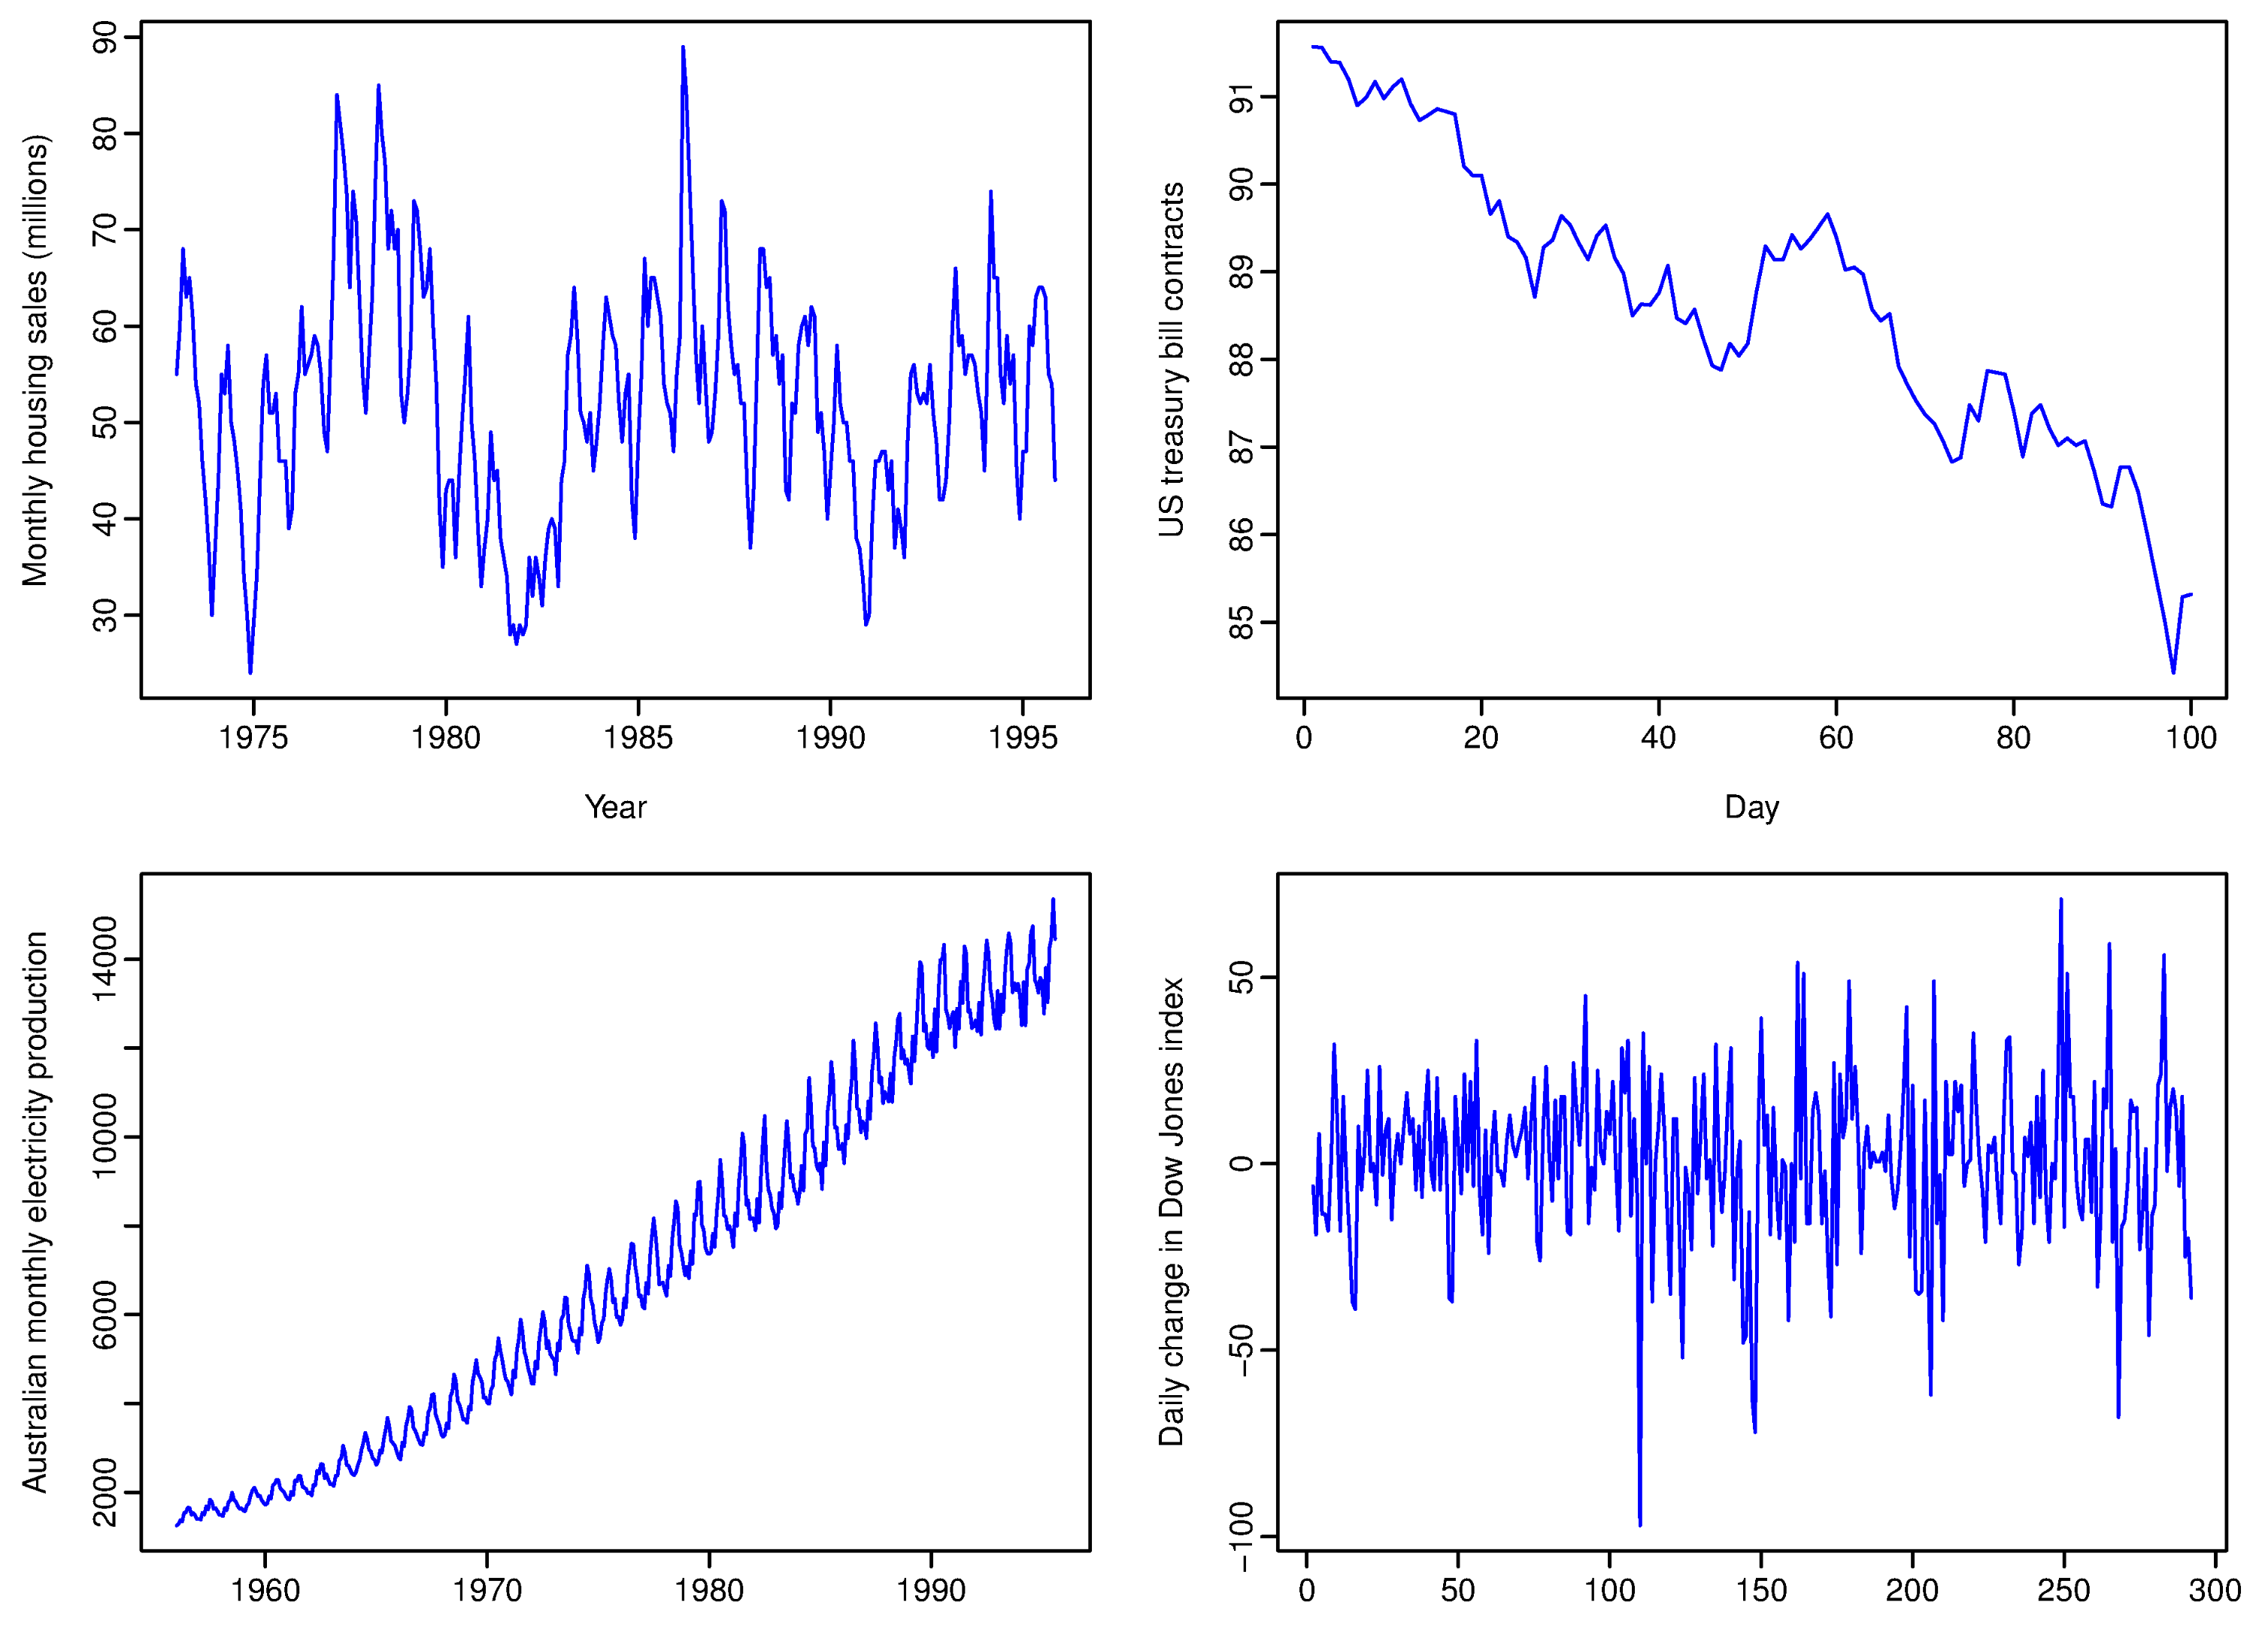
\includegraphics[width=1\linewidth]{lecture_2/fig/ts_components.png}
\end{figure}
\end{frame}
%=======
\begin{frame}{Стационарный временной ряд}
\textbf{Определение.} Временной ряд $\{x_i\}_{i=1}^{T}$ называется слабо стационарным (или стационарным в широком смысле), если
\begin{itemize}
    \item $\mathrm{E}[x_t]=$ const (т.е. временной ряд не имеет \textit{тренда}),
    \item $\mathrm{Cov}(x_t,x_{t+k}) = \mathrm{E}[(x_t - \mathrm{E}x_t)(x_{t+k} - \mathrm{E}x_{t+k})] = \gamma(k)$ (ковариация зависит только от разницы во времени).
\end{itemize}
Причем $\mathrm{Cov}(x_t,x_{t}) = \mathrm{D}(x_t) = \gamma(0) = \gamma_0$, т.е. дисперсия стационарного временного ряда не меняется со временем.
\begin{figure}
    \centering
    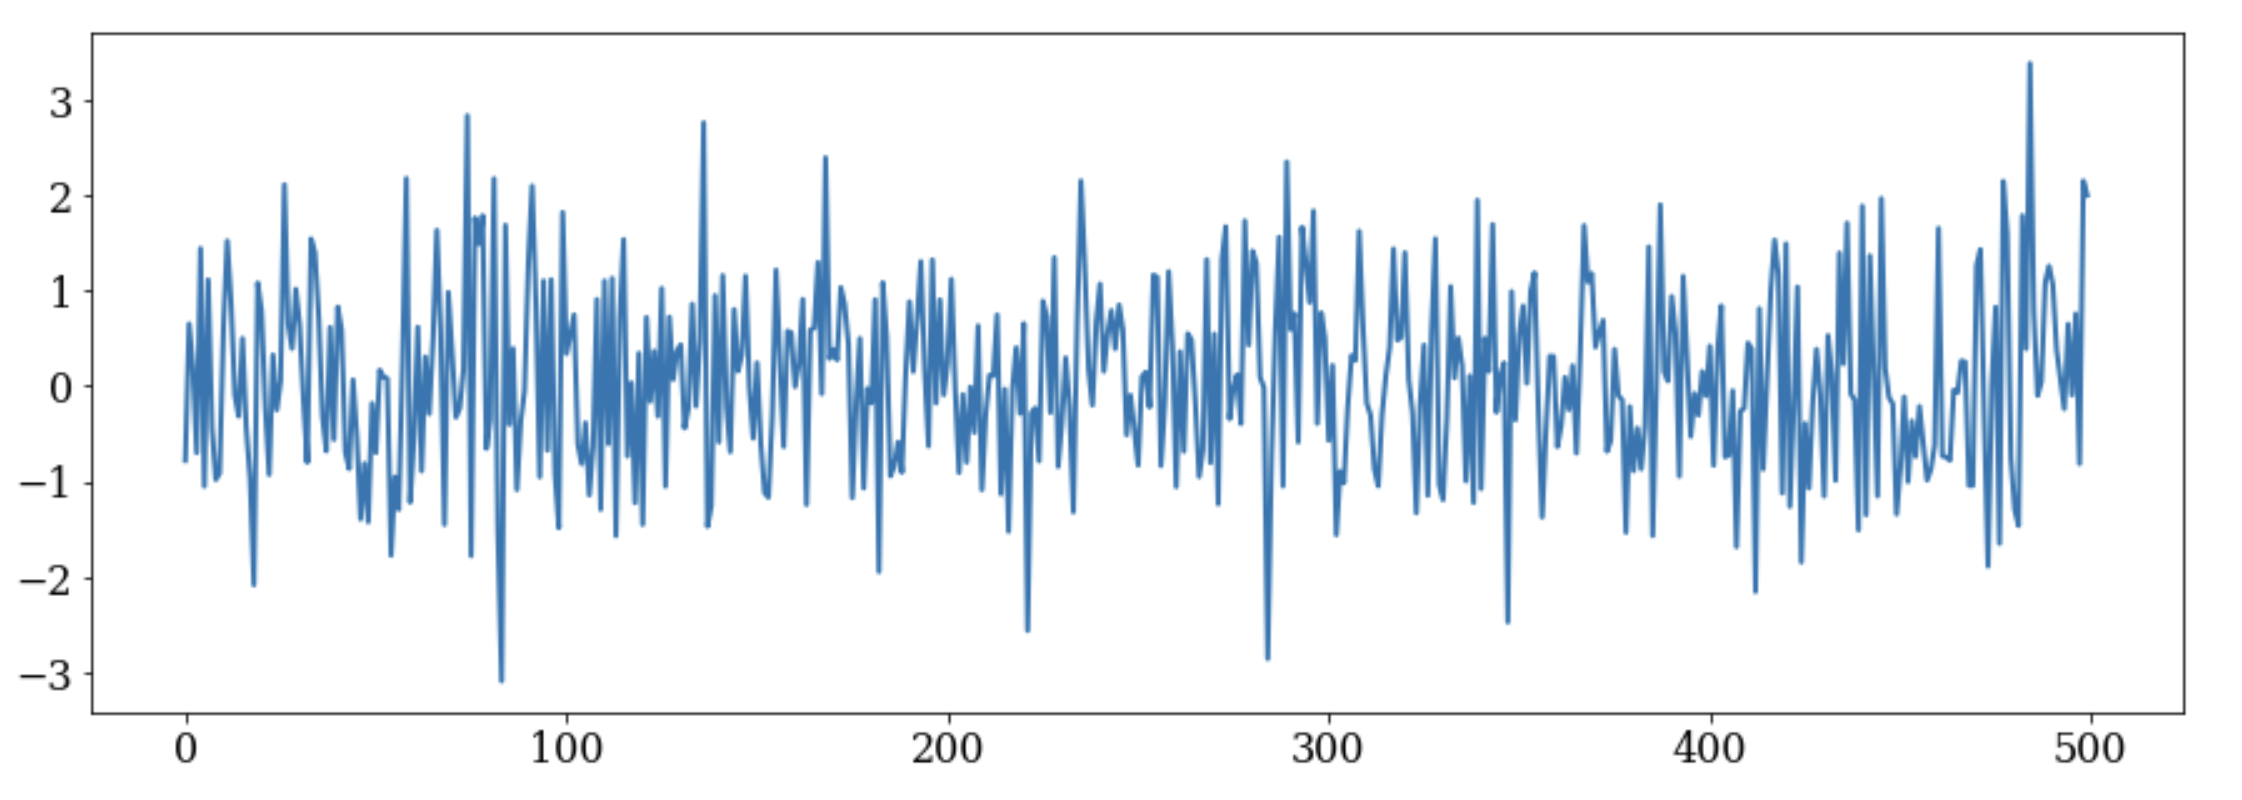
\includegraphics[width=0.9\linewidth]{lecture_2/fig/noise.png}
    \caption{Белый шум $u_t \sim \text{WN}(0, \sigma^2)$: $\mathrm{E}u_t = 0, \ \mathrm{D}u_t = \sigma^2, \ \mathrm{Cov}(u_t, u_{t + k}) = 0$}
\end{figure}
\end{frame}
%=======
\begin{frame}{Стационарный временной ряд}
\textbf{Вопрос}: какие из этих рядов стационарные?
\begin{figure}
    \centering
    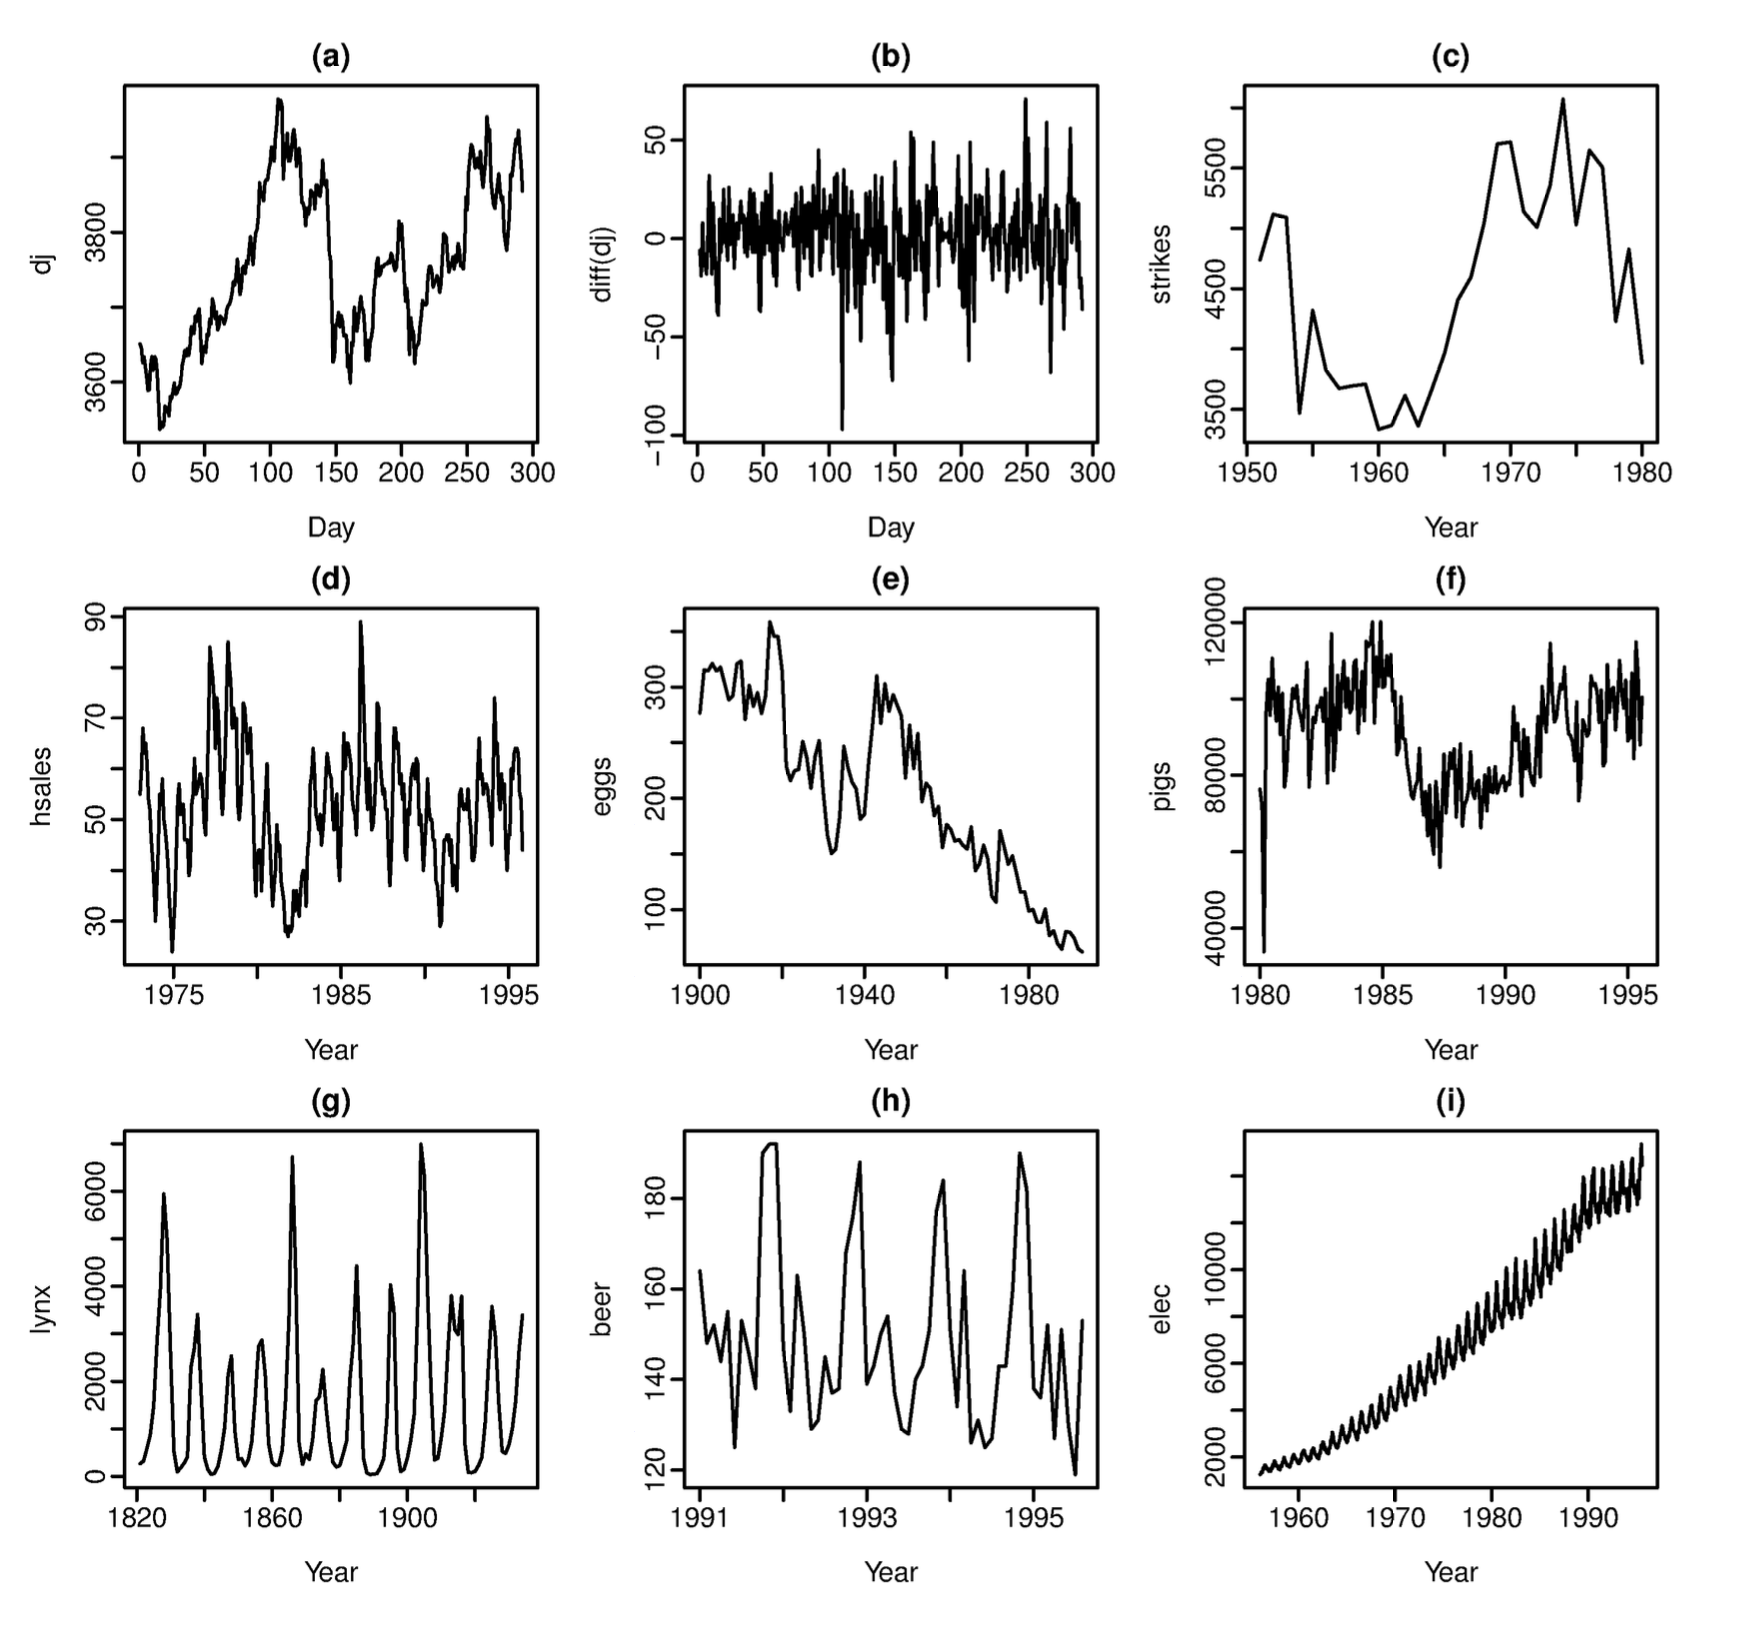
\includegraphics[width=0.8\linewidth]{lecture_2/fig/ts_stationary.png}
\end{figure}
\end{frame}
%=======
% \begin{frame}{Непараметрическая регрессия}
% \myfootnotewithlink{http://www.machinelearning.ru/wiki/images/archive/a/a2/20120416233549!Voron-ML-regression-slides.pdf}{сredit: http://www.machinelearning.ru/wiki/images/archive/a/a2/20120416233549!Voron-ML-regression-slides.pdf}
% \end{frame}
%=======
\begin{frame}{Автокорреляция}

\textbf{Определение.} Функция $\rho(k)$ называется  \textit{автокорреляционной функцией (autocorrelation function, ACF)} стационарного временного ряда.

\begin{equation*}
    \rho(k) = \mathrm{Corr}(x_t, x_{t+k}) = \frac{ \mathrm{Cov}(x_t,x_{t+k}) }{ \sqrt{ \mathrm{D}(x_t) \cdot \mathrm{D}(x_{t+k}) } } = \frac{ \gamma(k) }{ \sqrt{ \gamma(0) \cdot \gamma(0) } } = \frac{ \gamma(k) }{ \gamma(0)}
\end{equation*}
Оценка:
\begin{equation*}
    \hat{\rho}(k) = \frac{ \sum_{t=1}^{T-k}(x_t - \overline{x})(x_{t+k} - \overline{x})}{\sum_{t=1}^{T}(x_t - \overline{x})}, 
    \quad\text{где}\quad\overline{x} = \frac{1}{T}\sum_{t=1}^{T}x_t
\end{equation*}
Для стационарных временных рядов верно, что
\begin{equation*}
    \lim_{k \to \infty} \rho(k) = \infty
\end{equation*}

% \begin{figure}
%     \centering
%     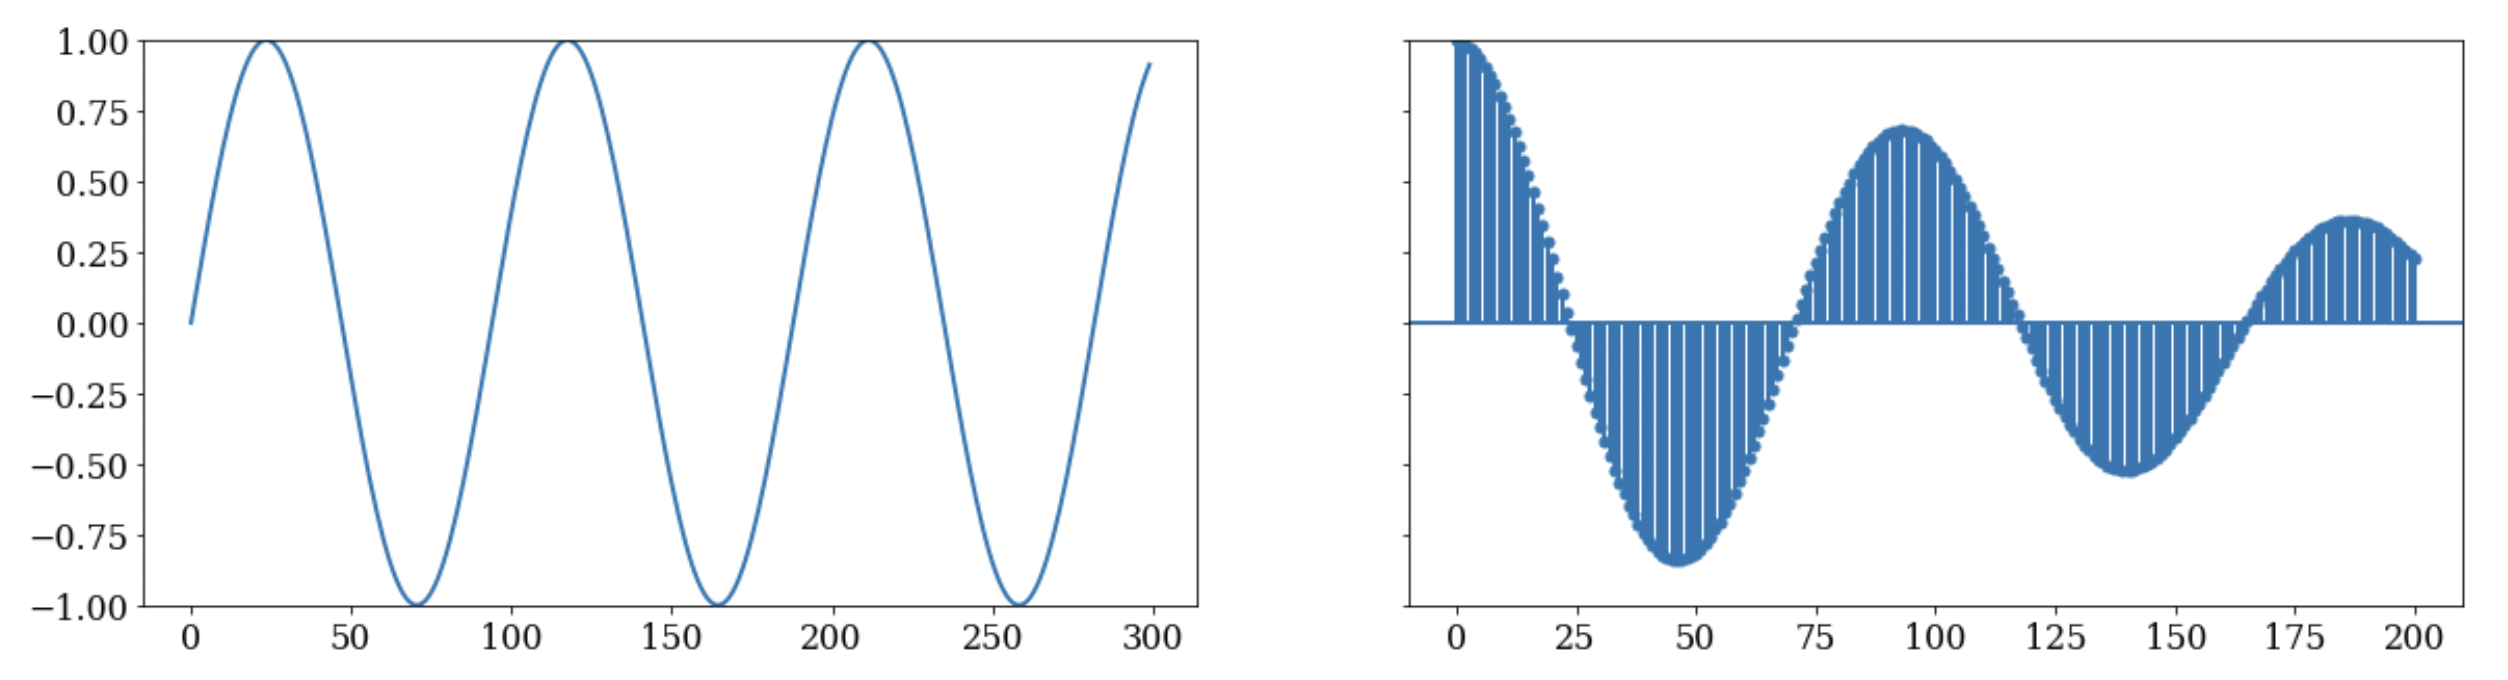
\includegraphics[width=1\linewidth]{lecture_2/fig/acf.png}
%     \caption{Периодический временной ряд и его коррелограмма}
% \end{figure}

\end{frame}
%=======
\begin{frame}{Автокорреляция}
\begin{figure}
    \centering
    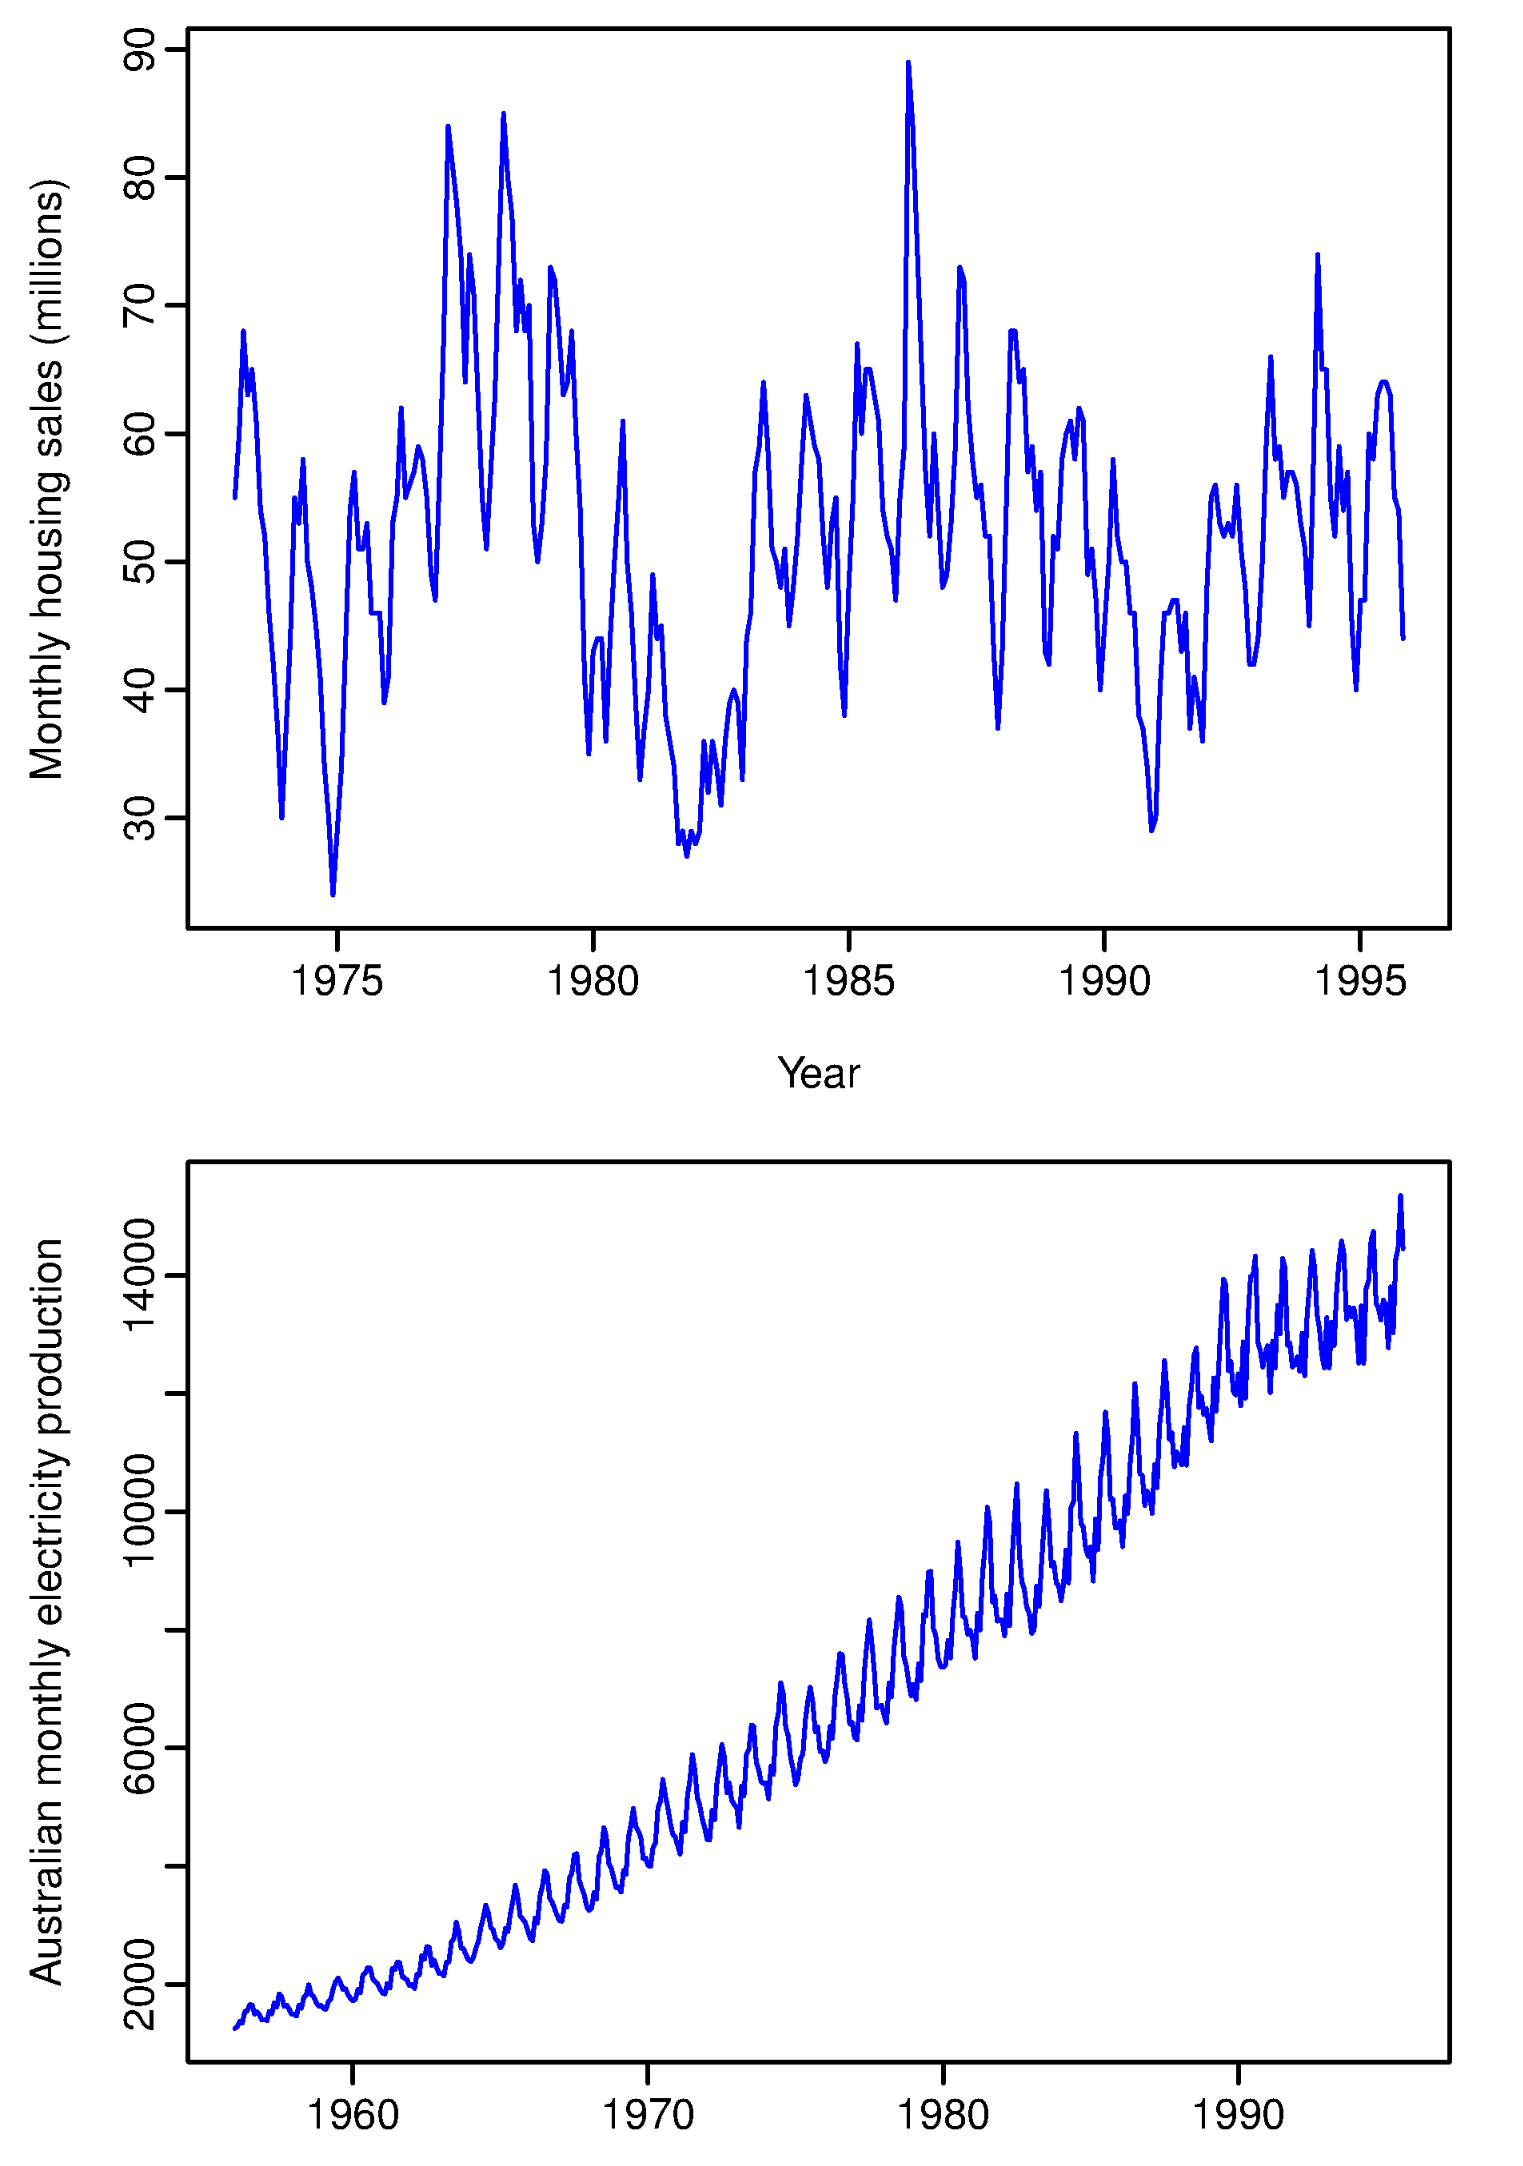
\includegraphics[width=0.45\linewidth]{lecture_2/fig/ts_components_1.png}
    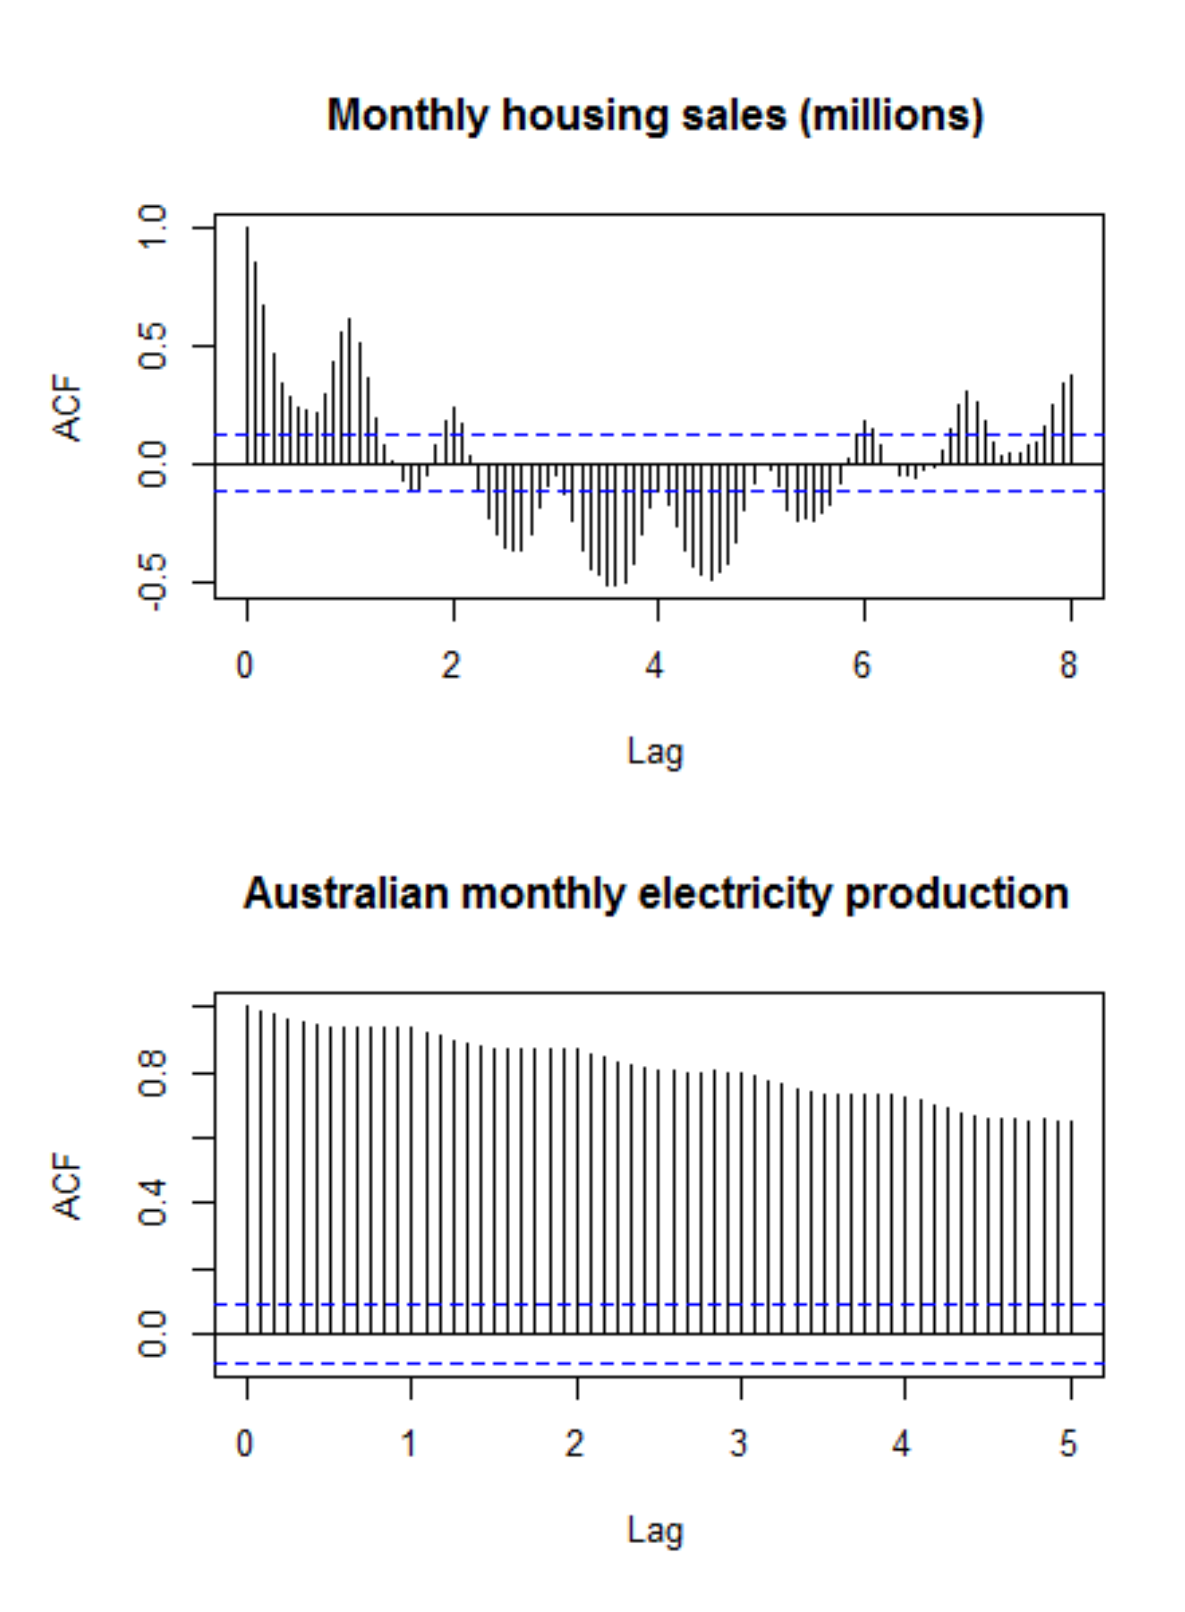
\includegraphics[width=0.53\linewidth]{lecture_2/fig/4acf_1.png}
\end{figure}
\end{frame}
%=======
\begin{frame}{Автокорреляция}
\begin{figure}
    \centering
    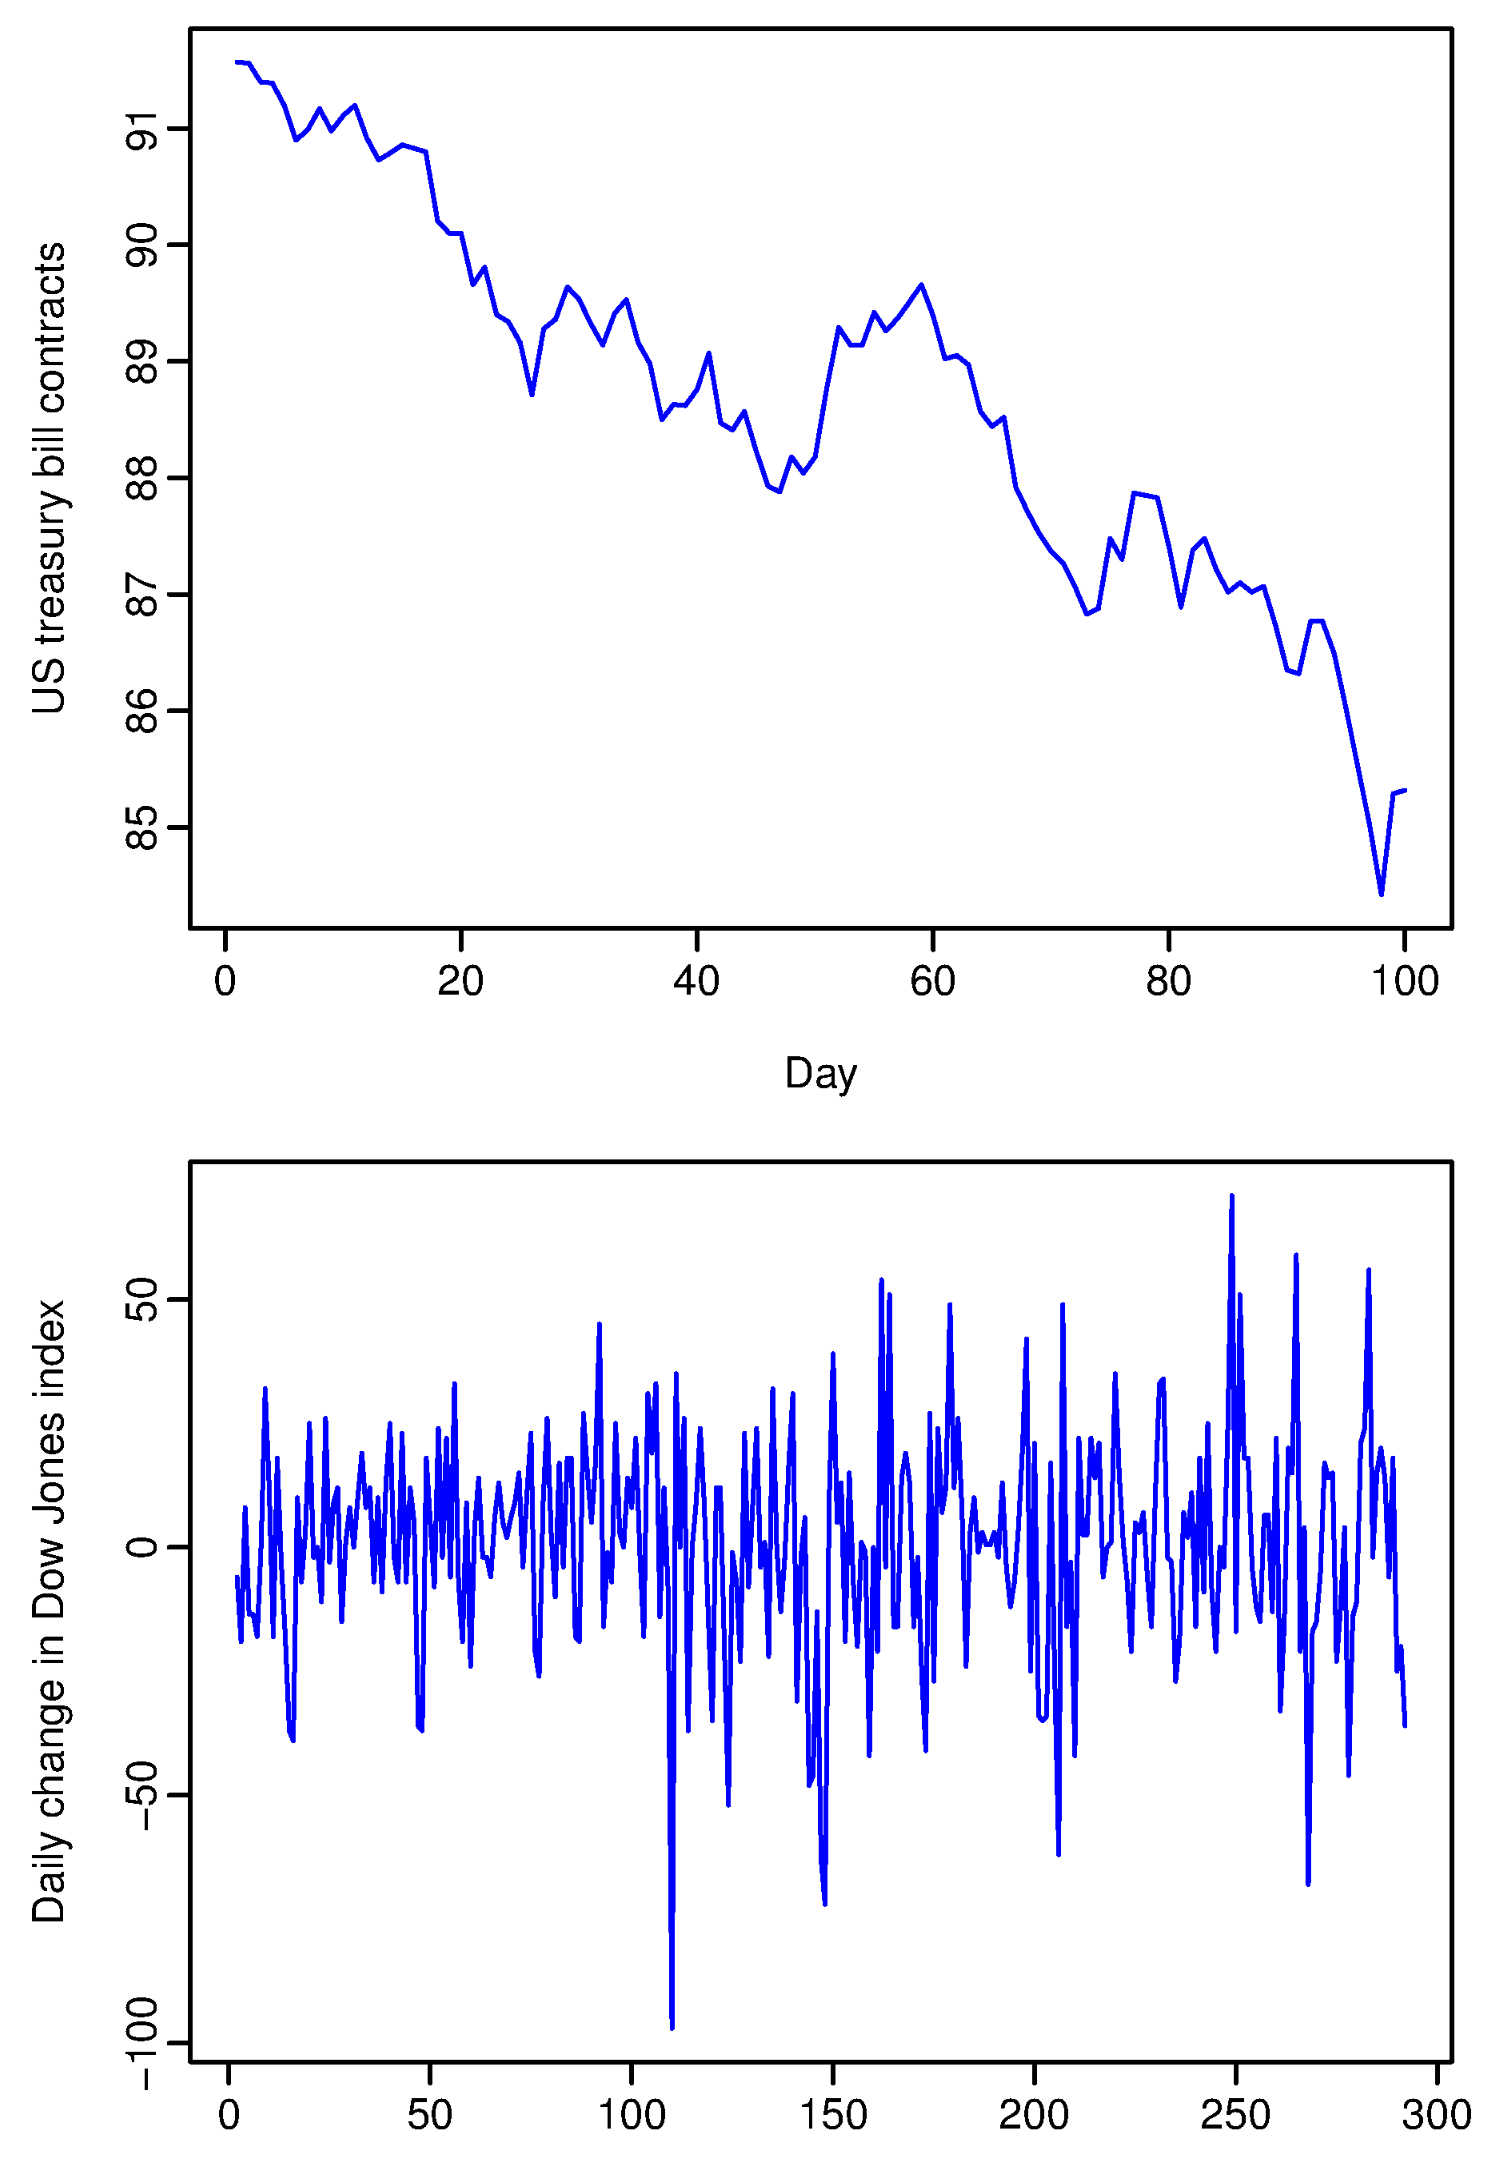
\includegraphics[width=0.45\linewidth]{lecture_2/fig/ts_components_2.png}
    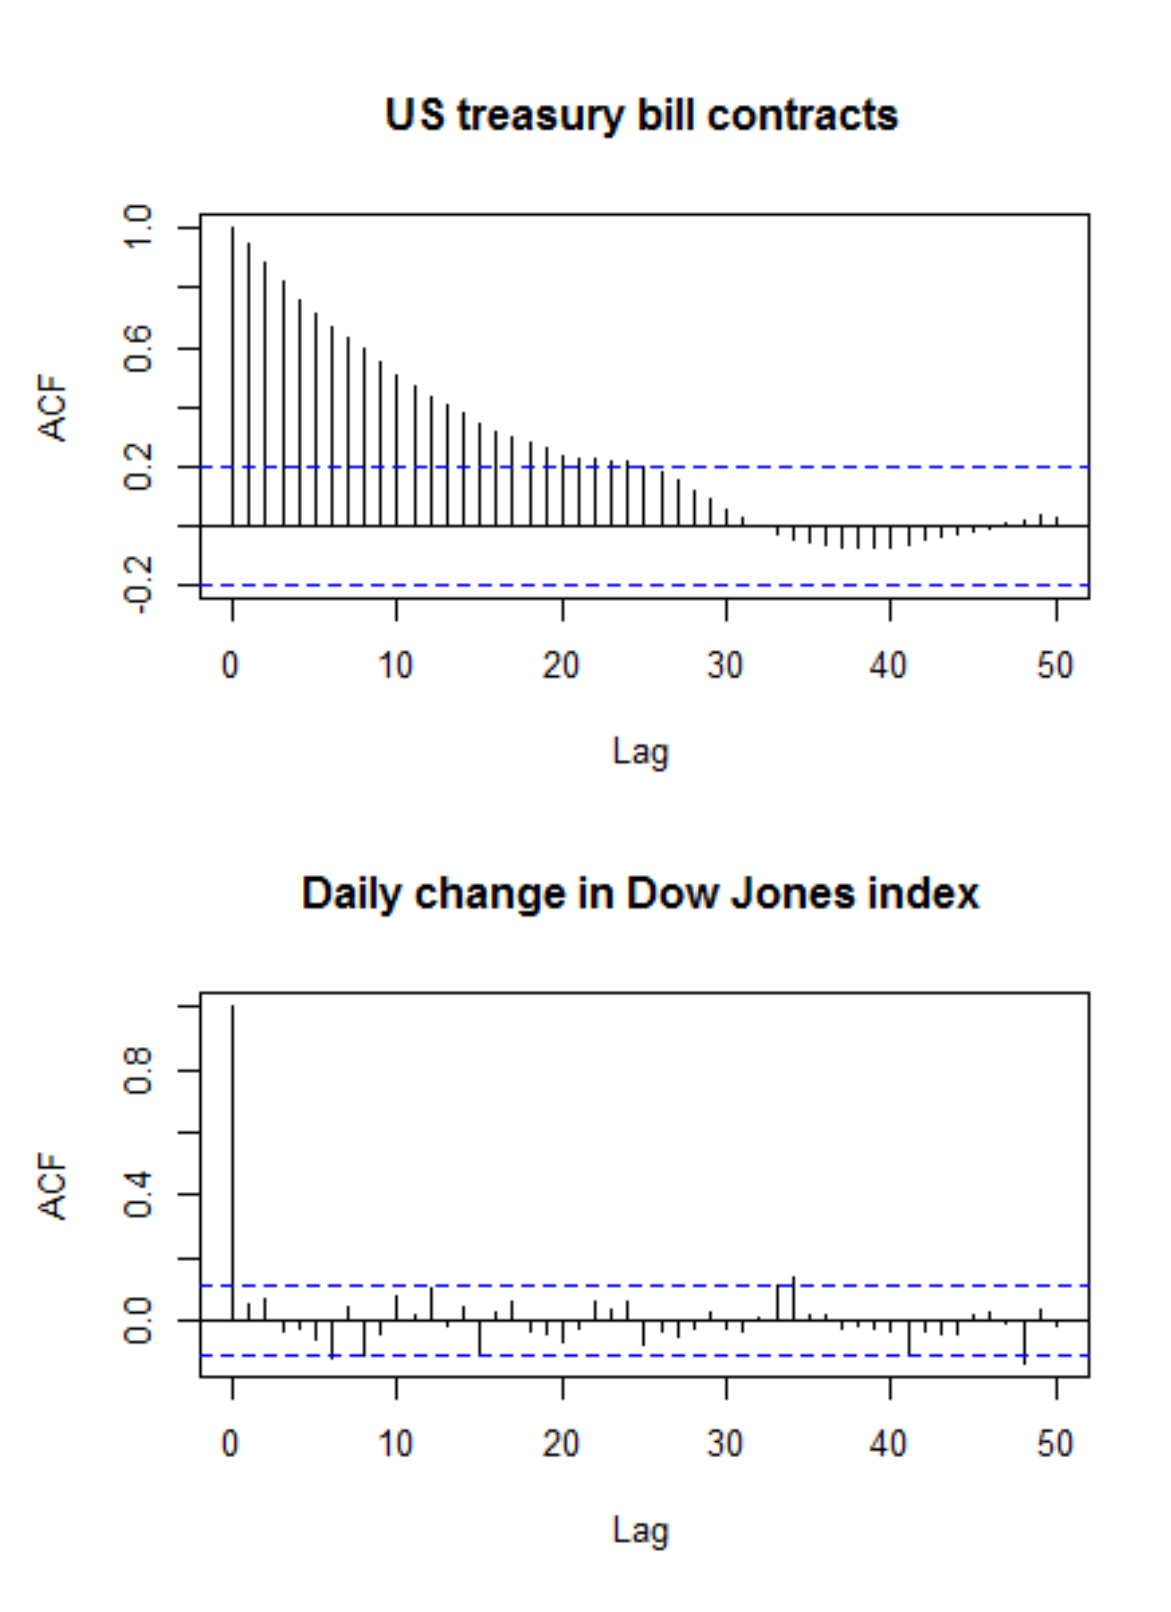
\includegraphics[width=0.53\linewidth]{lecture_2/fig/4acf_2.png}
\end{figure}
\end{frame}
%=======
\begin{frame}{Модель ARMA}
Общая смешанная модель ARMA$(p,q)$ (AutoRegression Moving Average) авторегрессии-скользящего среднего:
\begin{equation*}
x_t = \mu + \sum_{j=1}^{p}\phi_j x_{t-j} + u_t + \sum_{s=1}^{q}\theta_s u_{t-s},
\quad u_t \sim \text{WN}(0, \sigma^2),\quad  \phi_p,\theta_q \neq 0
\end{equation*}

\textbf{Составные части:}
\begin{itemize}
    \item $\mu + \sum_{j=1}^{p}\phi_j x_{t-j}$ --- авторегрессионная часть AR,
    \item $u_t + \sum_{s=1}^{q}\theta_s u_{t-s}$ --- часть скользящего среднего MA (в классическом случае гауссовский белый шум).
\end{itemize}
Согласно теорема Вольда, любой стационарный ряд может быть
аппроксимирован моделью ARMA$(p,q)$ с любой точностью.

\end{frame}

%=======
\begin{frame}{Модель ARMA. Прогноз}
\begin{equation*}
x_t = \mu + \sum_{j=1}^{p}\phi_j x_{t-j} + u_t + \sum_{s=1}^{q}\theta_s u_{t-s},
\quad u_t \sim \text{WN}(0, \sigma^2),\quad  \phi_p,\theta_q \neq 0
\end{equation*}

Пусть известны значения ряда $x_t$ и возмущения $u_t$ до момента времени $T$ включительно, а также получены веса $\phi_j$, $j = \overline{1, p}$, $\theta_s$, $s = \overline{1,q}$ модели ARMA$(p,q)$. \\
Выражение для $x_{T+1}$ в рамках модели:
\begin{equation*}
x_{T+1} = \mu + \sum_{j=1}^{p}\phi_j x_{T+1-j} + u_{T+1} + \sum_{s=1}^{q}\theta_s u_{T+1-s}
\end{equation*}
Неизвестным в правой части является только возмущение $u_{T+1}$. Отметим: $\mathrm{E}u_{T+1} = 0, \ \mathrm{Cov}(u_{T+1}, x_t) = 0$ для всех $t \leq T$. Оценка на момент времени $T+1$:
\begin{equation*}
\hat{x}_{T+1} = \mu + \sum_{j=1}^{p}\phi_j x_{T+1-j} + \sum_{s=1}^{q}\theta_s u_{T+1-s}
\end{equation*}

\end{frame}

%=======

%=======
\begin{frame}{Модель ARMA. Прогноз}

Выражение для $x_{T+2}$ в рамках модели:
\begin{equation*}
x_{T+2} = \mu + \sum_{j=1}^{p}\phi_j x_{T+2-j} + u_{T+2} + \sum_{s=1}^{q}\theta_s u_{T+2-s}
\end{equation*}
Неизвестными в правой части здесь является только возмущения $u_{T+1}, \ u_{T+2}$ и значение ряда $x_{T+1}$. Как и на предыдущем шаге, занулим неизвестные возмущения, а вместо значения $x_{T+1}$ используем его оценку $\hat{x}_{T+1}$, получим:
\begin{equation*}
\hat{x}_{T+2} = \mu + \phi_1 \hat{x}_{T+1} +  \sum_{j=2}^{p}\phi_j x_{T+2-j} + \sum_{s=2}^{q}\theta_s u_{T+2-s}
\end{equation*}

Заметим, что MA часть уменьшается с каждым последующим прогнозом в будущее.

\end{frame}

%=======

\begin{frame}{Модель ARMA. Прогноз}

Последовательное построение оптимального прогноза на $\tau$ шагов для общего случая:
\begin{enumerate}
    \item Записываем ARMA-формулу для $x_{T+\tau}$.
    \item Зануляем неизвестные возмущения $u_{T+1}, ..., u_{T+\tau}$.
    \item Заменяем неизвестные значения $x_{T+1}, ..., x_{T+\tau - 1}$ на их прогнозы, полученные на предыдущих шагах.
\end{enumerate}

\textbf{Вопросы}:
\begin{itemize}
    \item Как получить оптимальные веса модели ARMA?
    \item Как в реальных данных получить возмущения $u_t, \ t \leq T$, необходимые для построения прогноза? 
\end{itemize}

\end{frame}


%=======
\begin{frame}{Дифференцирование временного ряда}
\textbf{Дифференцирование ряда} — переход к попарным разностям его соседних
значений:
\begin{equation*}
x_1,...,x_T \rightarrow x_2',...,x_T',
\end{equation*}
\begin{equation*}
x_t' = x_{t} - x_{t-1} .
\end{equation*}

Дифференцированием можно стабилизировать среднее значение ряда и избавиться от тренда и сезонности.

Может применяться неоднократное дифференцирование; например, для второго порядка:
\begin{equation*}
x_1,...,x_T
\rightarrow
x_2^{'},...,x_T^{'}
\rightarrow
x_3^{''},...,x_T^{''},
\end{equation*}
\begin{equation*}
x_t^{''} = x_t^{'} - x_{t-1}^{'} = x_t - 2x_{t-1} + x_{t-2}.
\end{equation*}
\end{frame}
%=======
\begin{frame}{Дифференцирование временного ряда}
\textbf{Определение}: лаговый оператор $\mathrm{L}$ --- оператор сдвига, позволяющий получить значения элементов временного ряда на основании ряда предыдущих значений:
\begin{equation*}
    \mathrm{L}(x_t) \defeq x_{t-1}.
\end{equation*}
Далее $\mathrm{L}^2(x_t) = \mathrm{L}(\mathrm{L}(x_t)) = \mathrm{L}(x_{t-1}) = x_{t-2}.$
\vfill
Следовательно,  $\mathrm{L}^k(x_t) = x_{t-k}$, причем $\mathrm{L}^0(x_t) = x_{t}$.
\vfill
Тогда дифференцирование временного ряда представимо в виде
\begin{equation*}
    x_t' = x_{t} - x_{t-1} = ( 1 - \mathrm{L})(x_t).
\end{equation*}

\end{frame}
%=======
\begin{frame}{Дифференцирование временного ряда}
\begin{figure}
    \centering
    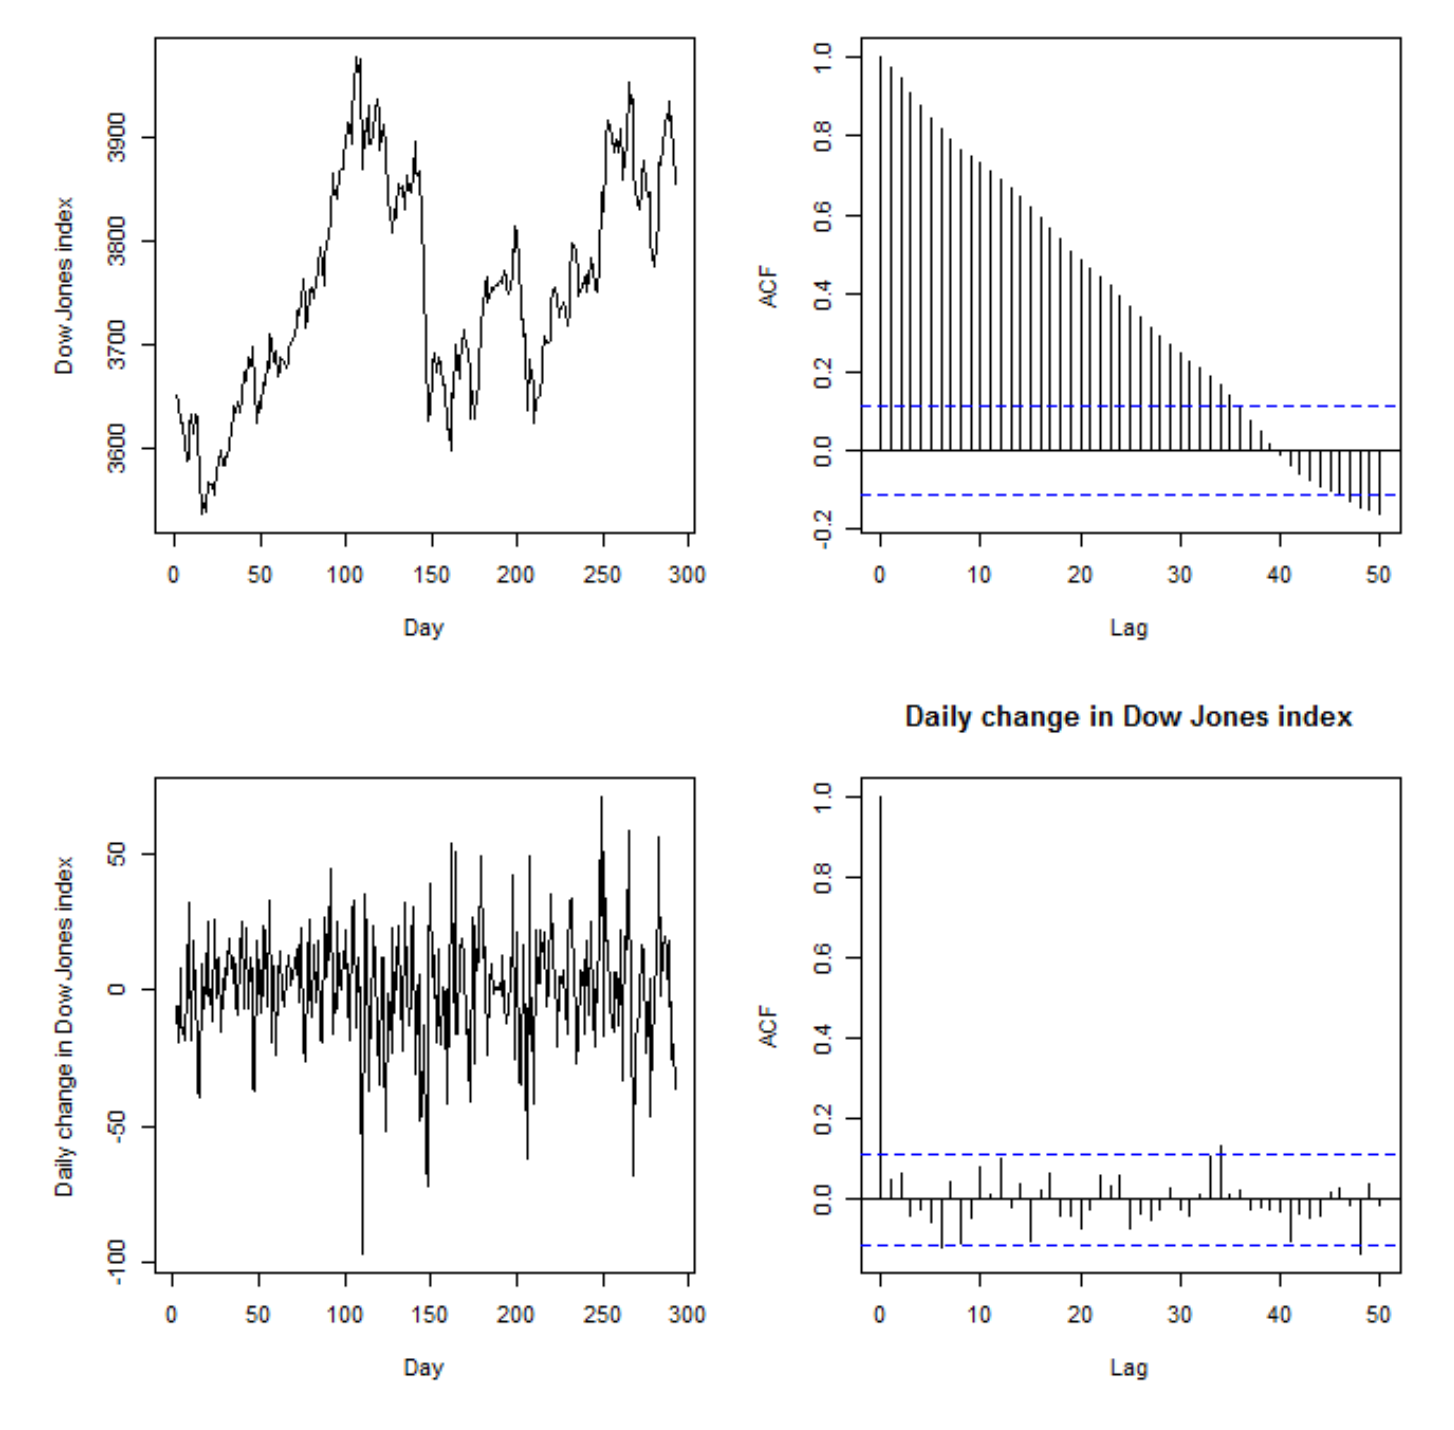
\includegraphics[width=0.75\linewidth]{lecture_2/fig/ts_diff.png}
\end{figure}
\end{frame}
%=======
\begin{frame}{Модель ARIMA}
Ряд описывается моделью ARIMA(p,d,q), если ряд его разностей
\begin{equation*}
\nabla^d x_t = (1 - \mathrm{L})^d(x_t)
\end{equation*}
описывается моделью ARMA(p,q):
\begin{equation*}
\nabla^d x_t = \mu + \sum_{j=1}^{p}\phi_j(\nabla^d x_{t-j}) + u_t + \sum_{s=1}^{q}\theta_s u_{t-s}.
\end{equation*}
\end{frame}
%=======
\begin{frame}{Модель Seasonal additive ARMA}
Для учета сезонной компоненты в моделью ARMA(p,q), добавляют авторегрессионные части и скользящее среднее по сезонным компонентам периода S.
\vfill
Модель ARMA(p,q):
\begin{equation*}
x_t = \mu + \sum_{j=1}^{p}\phi_j x_{t-j} + u_t + \sum_{s=1}^{q}\theta_s u_{t-s}
\end{equation*}
c авторегрессией с P сезонными компонентами:
\begin{equation*}
+ \phi_{S} x_{t-S}  + \phi_{2S} x_{t-2S} + ... + \phi_{PS} x_{t-PS}  
\end{equation*}
и с скользящим средним с Q сезоными компонентами:
\begin{equation*}
+ \theta_{S} u_{t-S} + \theta_{2S} u_{t-2S}  + ... + \theta_{QS} u_{t-QS}.
\end{equation*}
\end{frame}
%=======
\begin{frame}{Модель SARIMAX}
К модели SARIMA(p,d,q)(P,D,Q) добавляюся \textit{экзогенные}переменные, значение которых формируется вне модели.
Экзогенные переменные являются в модели независимыми величинами, а их изменение называется автономным изменением.
\begin{equation*}
x_t = \mu + \sum_{j=1}^{p}\phi_j x_{t-j} + u_t + \sum_{s=1}^{q}\theta_s u_{t-s} +...+ \textcolor{red}{\sum_{i=1}^{r}\beta_i x^{\text{exog}}_i}
\end{equation*}

\end{frame}

%=======
\begin{frame}{Модель SARIMAX}
Из документации statsmodels.tsa.statespace.sarimax.SARIMAX Python:
\begin{figure}
    \centering
    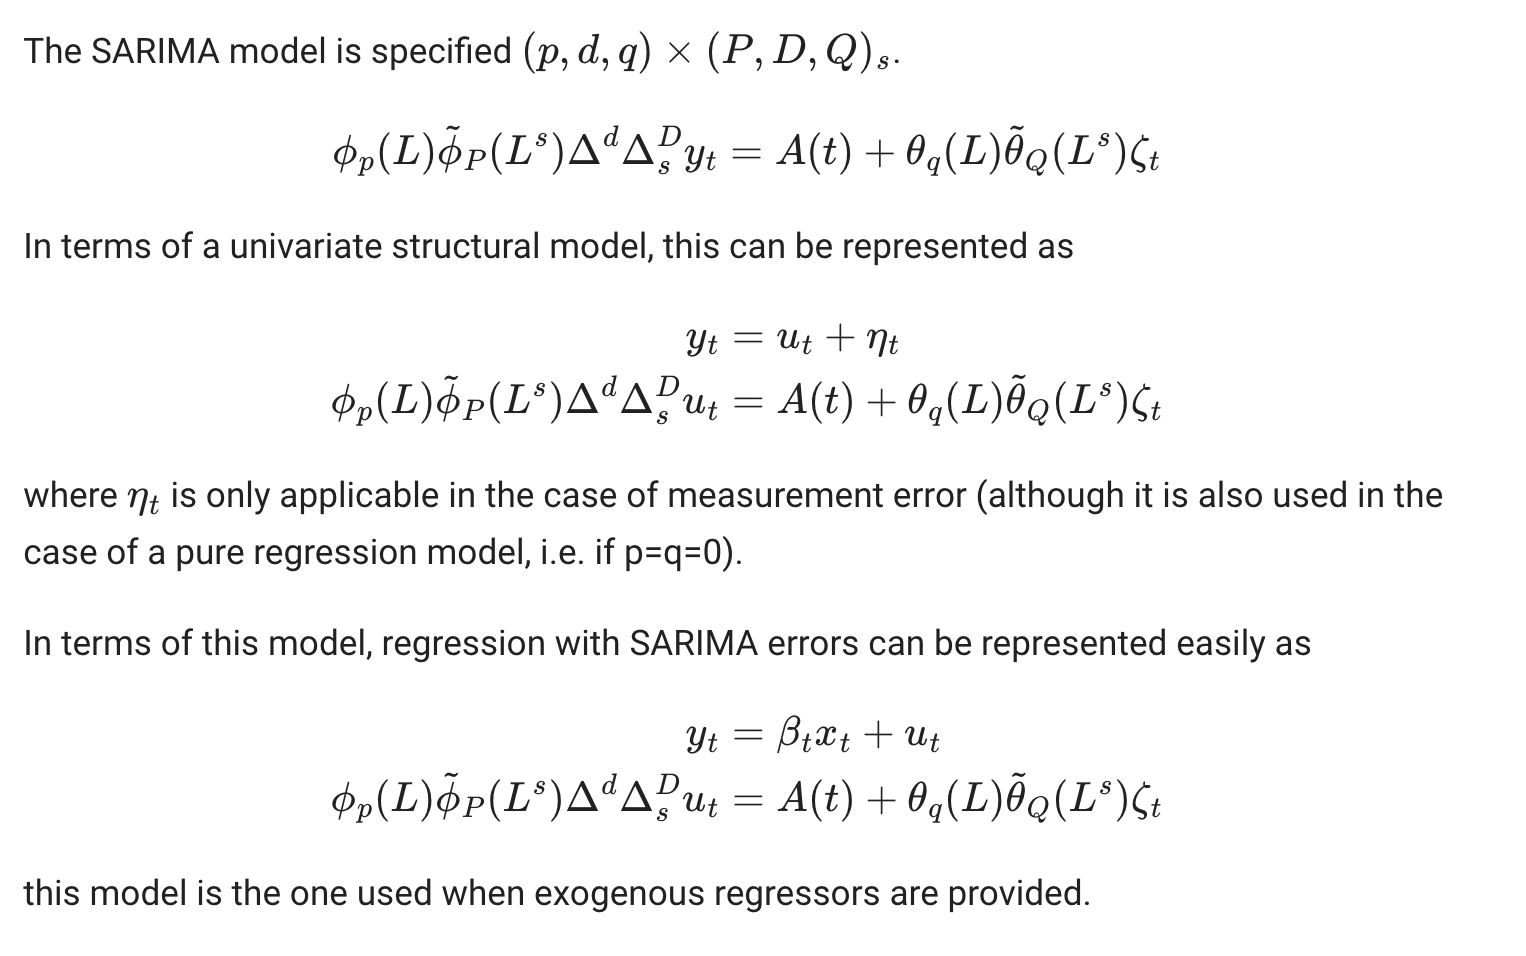
\includegraphics[width=0.75\linewidth]{lecture_2/fig/sarimax_tsa.png}
\end{figure}
\myfootnotewithlink{https://www.statsmodels.org/dev/generated/statsmodels.tsa.statespace.sarimax.SARIMAX.html}{сredit: https://www.statsmodels.org/dev/generated/
statsmodels.tsa.statespace.sarimax.SARIMAX.html}
\end{frame}
%=======
\begin{frame}{Информационные критерии}
\textbf{Критерий Акаике (Akaike's information criterion, AIC)} --- критерий выбора из класса параметризованных регрессионных моделей, оценивающий модели с разным числом параметров.
Содержит функцию штрафа, линейно зависящую от числа параметров
\begin{equation*}
    AIC = 2\frac{p + q}{T} + \ln\Bigg(\frac{\sum_{t=1}^T (x_t - \hat{x}_t)^2}{n}\Bigg)
\end{equation*}

\end{frame}
%=======
\begin{frame}{Прогнозирование с помощью ARIMA}
\begin{enumerate}
    \item Строится график ряда, идентифицируются необычные значения.
    \item При необходимости делается стабилизирующее дисперсию
    преобразование.
    \item Если ряд нестационарен, подбирается порядок дифференцирования.
    \item Анализируются ACF/PACF, чтобы понять, можно ли использовать модели AR($p$)/MA($q$).
    \item Обучаются модели-кандидаты, сравнивается их AIC.
    \item Остатки полученной модели исследуются на несмещённость, стационарность и неавтокоррелированность; если предположения не выполняются, исследуются модификации модели.
    \item В финальной модели $t$ заменяется на $T + \tau$, будущие наблюдения — на их прогнозы, будущие ошибки — на нули, прошлые ошибки — на остатки.
\end{enumerate}
\end{frame}
%=======
\begin{frame}{Резюме}
    \begin{itemize}
        \item временные ряды представляются как случайные процессы,
        \item стационарный временной ряд по Теореме Вольда предстваим с помощью ARMA модели,
        \item модель ARMA --- линейная комбинация предыстории и шумов,
        \item модель SARIMAX --- это объединение авторегрессии с некоторыми эвристиками  (сезонность, тренд) для обеспечения стационарности временного ряда.
        
    \end{itemize}
\end{frame}

\end{document} 